%%%%%%%%%%%%%%%%%%%%%%%%%%%%%%%%%%%%%%%%%
% Stylish Article
% LaTeX Template
% Version 2.1 (1/10/15)
%
% This template has been downloaded from:
% http://www.LaTeXTemplates.com
%
% Original author:
% Mathias Legrand (legrand.mathias@gmail.com) 
% With extensive modifications by:
% Vel (vel@latextemplates.com)
%
% License:
% CC BY-NC-SA 3.0 (http://creativecommons.org/licenses/by-nc-sa/3.0/)
%1
%%%%%%%%%%%%%%%%%%%%%%%%%%%%%%%%%%%%%%%%%

\documentclass[fleqn,10pt]{SelfArx} % Document font size and equations flushed
% left

\usepackage[english]{babel} % Specify a different language here - english by default

\usepackage{marvosym, epigraph, subfig, listings, microtype}

\usepackage[sortcites=false,style=authoryear-comp,bibencoding=utf8, natbib=true, firstinits=true, maxcitenames=2, maxbibnames = 99, uniquename=false, backend=bibtex, useprefix=true, backref=false,doi=false,isbn=false,url=false,dashed=true]{biblatex}
\setlength\bibhang{20pt}
\bibliography{references.bib}
\AtEveryBibitem{%
	\clearfield{day}%
	\clearfield{month}%
	\clearfield{endday}%
	\clearfield{endmonth}%
}

%----------------------------------------------------------------------------------------
%	COLUMNS
%----------------------------------------------------------------------------------------

\setlength{\columnsep}{0.55cm} % Distance between the two columns of text
\setlength{\fboxrule}{0.75pt} % Width of the border around the abstract

%----------------------------------------------------------------------------------------
%	COLORS
%----------------------------------------------------------------------------------------

\definecolor{color1}{RGB}{0,0,90} % Color of the article title and sections
\definecolor{color2}{RGB}{0,20,20} % Color of the boxes behind the abstract and headings

%----------------------------------------------------------------------------------------
%	HYPERLINKS
%----------------------------------------------------------------------------------------

\usepackage{hyperref} % Required for hyperlinks
\hypersetup{hidelinks,colorlinks,breaklinks=true,urlcolor=color2,citecolor=color1,linkcolor=color1,bookmarksopen=false,pdftitle={Housing market and migration revisited: a Bayesian multilevel gravity model for Dutch municipalities},pdfauthor={Thomas de Graaff}}

%----------------------------------------------------------------------------------------
%	ARTICLE INFORMATION
%----------------------------------------------------------------------------------------

\JournalInfo{Journal of Regional Science} % Journal information
\Archive{Working paper} % Additional notes (e.g. copyrigh, DOI, review/research article)

\PaperTitle{Urban exodus: housing market structure and interregional migration revisited}

\Authors{Thomas de Graaff\textsuperscript{1}*} % Authors
\affiliation{\textsuperscript{1}\textit{Department of Spatial Economics, Vrije Universiteit Amsterdam, Amsterdam, The Netherlands}} % Author affiliation
\affiliation{*\textbf{Corresponding author}: \Letter{} t.de.graaff@vu.n; \Mundus{} \href{thomasdegraaff.nl}{thomasdegraaff.nl}} % Corresponding author

\Keywords{Gravity model --- housing market --- interregional migration --- multilevel model --- cities}
\newcommand{\keywordname}{Keywords} 

%%----------------------------------------------------------------------------------------
%%	ABSTRACT
%%----------------------------------------------------------------------------------------

\Abstract{This paper addresses the impact of home-ownership and social renting
  rates on intercity residential migration in the Netherlands. It especially
  focuses on their role on the migration of natives out of the larger and
  popular Dutch cities. By applying a
  Bayesian multilevel gravity model I control simultanously for (\emph{i}) both
  city-specific effects of origin and destination, (\emph{ii}) dyad-pair
  specific effects, and (\emph{iii}) the impact of the housing market structure
  in both the city of origin and the city of destination. I find positive and
  high elasticities of social renting (0.8) and homeownership (1.8) rates on
  out-migration, while homeownership rates have a smaller and negative impact
  ($-0.5$) on in-migration. Moreover, city specific in- and out-migration flows
  are highly correlated (0.88) just as dyad-specific flows (0.8). Finally, I
  show that my probabilistic model is able to accurately predict migration flows
  both within and out-of-sample.}

%----------------------------------------------------------------------------------------
\hypersetup{draft} 
\begin{document}

\flushbottom
\maketitle
\thispagestyle{empty}

%----------------------------------------------------------------------------------------

\section{Introduction}

In the recent decade cities have been proclaimed to be the overall ``winners''
within the regional economic landscape \citep[]{glaeser2012triumph}. Indeed,
there is a large empirical literature that finds that especially large cities exhibit relatively more employment, more innovation and produce overall more added value \citep[see, e.g.,][]{balland2020complex}. Most of this success of (large) cities can be attributed to positive regional and urban agglomeration economies \citep[see for a recent overview of the size, scope and nature of these urban economies][]{duranton2020, rosenthal2020}

Arguably, however, urban succes does not accrue to everyone and recent research has shown as well the negative aspects of this success.

\begin{figure*}[h!]\centering % Using \begin{figure*} makes the figure take up
  % the entire width of the page
 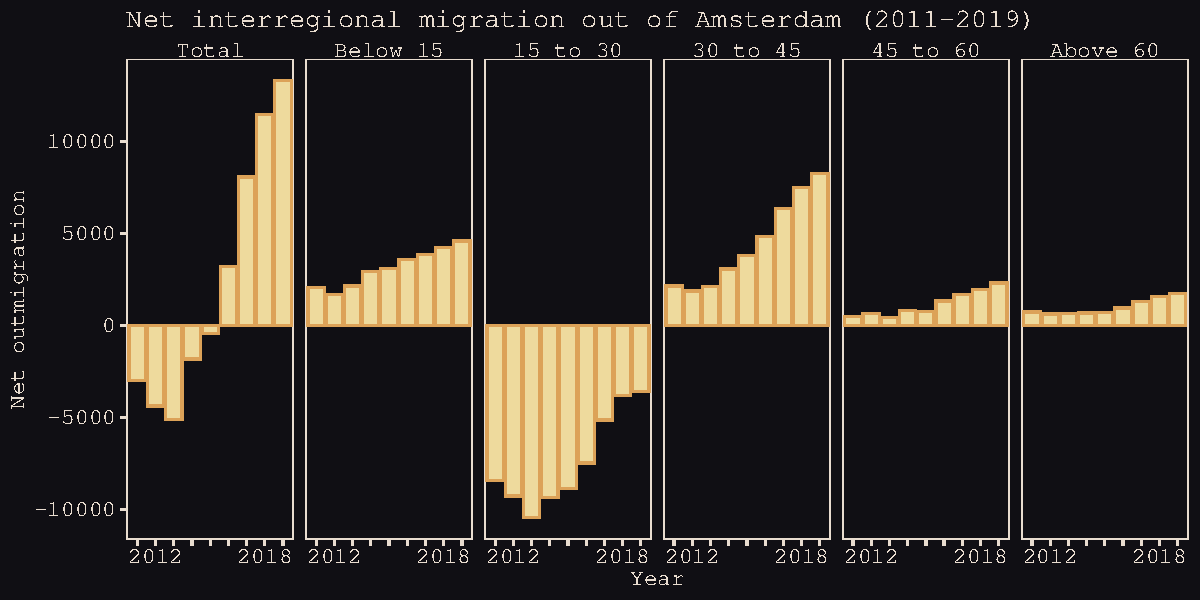
\includegraphics[width=1\linewidth]{../../fig/outmig_amsterdam.pdf}
  \caption{Interregional migration out of Amsterdam in the period 2011-2019 for various age cohorts (including total out-migration in the most left-panel)}
  \label{fig:adam_mig}
\end{figure*}

To anticipate the results of this paper, I find strong negative effects of
home-ownership rates on on both in- and out-migration flows. Further, social
renting rates also affect regional migration flows negatively, but only for
out-migration.

This paper reads as follows. The next section describes the data and focuses
especially on the distribution of regional migration flows and housing market
structure. Section 3 describes the modelling approach, where starting from
traditional gravity model and using the descriptives of the migration flows, a
Bayesian multilevel gravity model is constructed. Section 4 gives both the model
results and interprets them by providing as well predictions within and
out-of-sample. The last section concludes.

 \section{Data}

 \begin{figure*}[t!]\centering % Using \begin{figure*} makes the figure take up
% the entire width of the page
   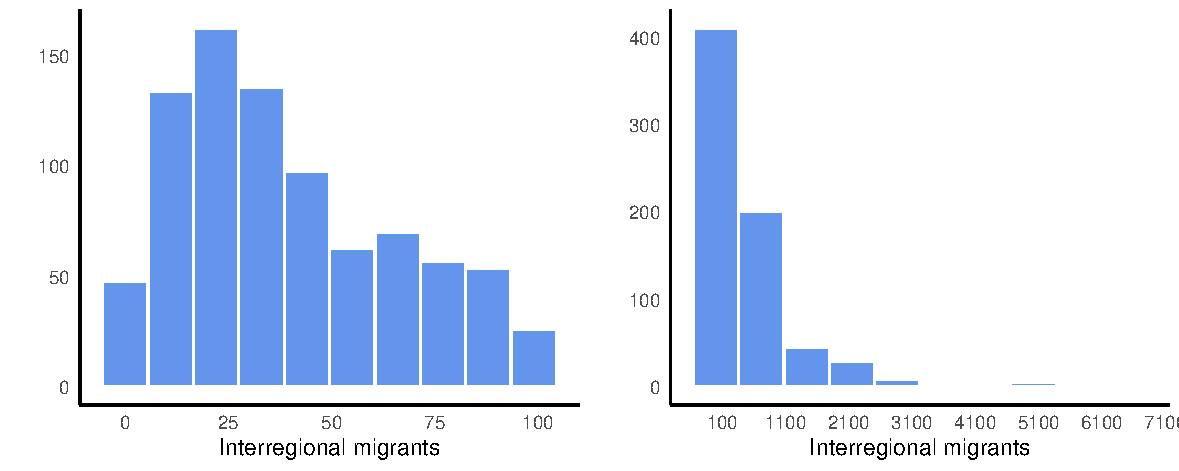
\includegraphics[width=0.8\linewidth]{./../../fig/hist_mig_corop.pdf}
          \caption{Histogram of inter-regional migrant flows. Left panel shows the histogram of
small migrant flows ($0 \leq N < 100$) and the right panel shows the histogram of
large migrant flows ($N \geq 100$). Note the different scale of the y-axes.}
          \label{fig:hist_mig_corop}
        \end{figure*}

I use inter-regional migration flows measured in individuals between
all of the 40 Dutch COROP regions between 2012 and 2018. I use no information on
within regional migration. So, I have 320 regional
characteristics (or doubled when accounting for both origin and destination
municipalities) and 10,902 aggregate migration flows ($7 \times (40 \times 40 - 40)$).

The histograms in Figure \ref{fig:hist_mig_corop} show the distribution of
migrant flows within my sample. The left panel deals with migrant flows below
100, the right panel with migrant flows of 100 and larger. Two main observations
can be made.

\section*{Acknowledgments}

I would like to thank Wim Bernasco, Thor Husby, Viktor Venhorst, Maureen
Lanhuizen, participants at the 15$^{\text{th}}$ biennial NECTAR conference in
Helsinki, participants at the 59$^{\text{th}}$ ERSA conference in Lyon and
seminar participants at the VU University Amsterdam for valuable comments on a
first draft of this paper. Paper, data and code can be retrieved from the
following project's GitHub page:

\href{https://github.com/Thdegraaff/migration_gravity}{https://github.com/Thdegraaff/migration\_gravity}.

%----------------------------------------------------------------------------------------
%	REFERENCE LIST
%----------------------------------------------------------------------------------------

\addcontentsline{toc}{section}{references} % Adds this section to the table of contents
\printbibliography

%----------------------------------------------------------------------------------------

\end{document}
%%% Local Variables:
%%% mode: latex
%%% TeX-master: t
%%% End:
